\section{Interface - Asym. Cipher}

\begin{frame}

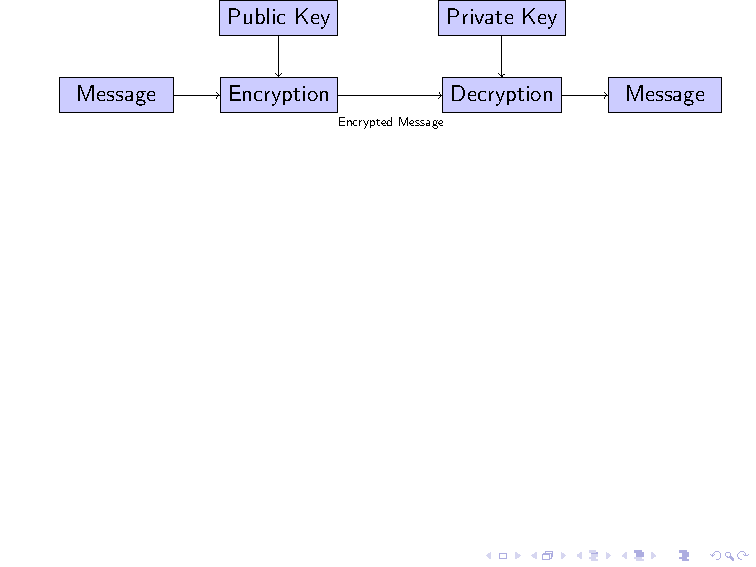
\includegraphics[trim=0.5cm 6cm 14cm 0cm, height=3.5cm]{figures/asym_cipher.pdf}


\begin{itemize}
  \small{
  \item Public and private key created by one person
  \item Public key sended to everyone who wants to get a communication
  \item Private key stay by who has created the key pair
  \item Public key allows the Encryption of the message
  \item Private key only can decrypt the message
  \item Allows privacy (only this one who has the private key can decypt the
  messages)
  \item Integraty (Sure that nobody can modify the messages during the
  transfer) }
\end{itemize}



\end{frame}
